\chapter{Hardvér}

\label{kap:hardver} % id kapitoly pre prikaz ref

V tejto kapitole popíšeme a rozoberieme podstatné aspekty zvoleného hardvéru. Pri útokoch pomocou indukovania chýb je často potrebná vysoká presnosť časovania v stovkách až desiatkach nanosekúnd. Lacnejší hardvér často takúto presnosť nie je schopný dosiahnuť. Hlavným cieľom tejto práce je overiť túto skutočnosť a zistiť akú presnosť časovania dokáže takýto hardvér poskytnúť. Finančné náklady na všetky súčiastky použité pri implementovaných útokoch sa pohybujú rádovo v desiatkach eúr.

\section{ATMega328P}
Najdôležitejším zariadením pre účely tejto práce je Atmel mikrokontrolér s osem bitovou architektúrou AVR, dnes vlastnený firmou Microchip Technology Inc. Tento mikrokontrlér je súčasťou viacerých modelov vývojových dosiek Arduino, ktoré sú často využívané pri vývoji jednoduchých vnorených zariadení. Zároveň zvykne byť použitý aj pri nasadení skutočných produktov, najmä vnorených systémov s nízkou spotrebou. Mikrokontrolér ATMega328P bol aj preto zvolený ako cieľom útokov implementovaných v tejto práci, ale hlavným dôvodom bola jeho veľmi nízka cena pohybujúca sa okolo desať eúr. Techniky útokov použité v tejto práci môžu s nezanedbateľnou pravdepodobnosťou trvalo poškodiť cielený hardvér, preto sme sa rozhodli použiť viacej rovnakých čipov. Konkrétne boli testované štyri exempláre formátu ATMega328P-PU z dvoch (po dvojiciach) rôznych sérií výroby. Okrem toho bol použitý aj ako zdroj útokov generujúci raidiace impulzy do rôznych obvodov využívajúcich niektoré techniky spomenuté v kapitole \ref{kap:teoria}, konkrétne ako súčasť dosky Adrunino Nano.

\subsection{Kľúčové vlastnosti}
Zvolený formát čipu ATMega328P-PU je v púzdre THT (Through Hole Technology), čo znamená, že piny na čipe sú vyvedené vo forme \uv{kolíkov} a je možné čip zapojiť bez potreby pájkovania pomocou nepájivého kontaktného poľa (angl. solderless breadboard). Takéto zapojenie potom možno jednoducho a bezprostredne modifikovať počas experimentovania. Ďalšou vlastnosťou je možnosť pripojenia externého oscilátora s frekvenciou maximálne 16 MHz, čo znamená väčšiu flexibilitu nastaviteľných parametrov jednotlivých útokov. Na čipe sa nachádza aj interný oscilátor s frekvenciou 8 MHz a možno ho využiť miesto zapojenia s externým \cite{atmegaData}.

Čo sa týka softvéru, pre programovanie mikrokontroléra ATMega328P potrebujeme kompilátor nízko-úrovňového jazyka (napríklad C) pre architektúru AVR. Nahratie programu do trvácnej flash-pamäte na mikrokontroléri možno zabezpečiť napríklad pomocou ISP (In-System Programming) programátora. Pre tento účel, je potrebné, aby na mikrokontroléri bol prítomný zavádzací program (angl. bootloader), ďalej len zavádzač, ktorý dokáže komunikovať s ISP programátorom. Jednoduchý a automatizovaný spôsob pre vykonanie týchto operácií poskytuje aj integrované vývojové prostredie (IDE) Arduino IDE, ktoré sme sa rozhodli použiť. Arduino IDE interne používa kompilátor AVR-GCC a ISP programátor AVRDUDE, ktoré sú voľne dostupné aj samostatne.

\subsection{Architektúra AVR}
Mikrokontrolér ATMega328P implementuje osem bitovú architektúru AVR. Niektoré aspekty tejto architektúry sú dôležité pre pochopenie niektorých častí kódu písaných v asembleri v rámci tejto práce, preto ich stručne opíšeme. AVR je zaraďovaná do triedy RISC (Reduced Instruction Set Computer) architektúr \cite{avrInstruction}. Poskytuje tridsaťdva (R0 -- R31) osembitových všeobecných registrov, z nich niektoré so špeciálnym významom pri vybraných inštrukciách. V tejto práci používame tieto registre len v základnom, všeobecnom význame. Pre prístup do pamäte slúžia dve základné inštrukcie LD (Load), ST (Store) a ich varianty. 

Ovládanie GPIO (General Purpose Input Output) pinov na mikrokontroléri je zabezpečené pomocou špeciálnych vstupno-výstupných registrov. Každý pin má priradený jeden zo štyroch tzv. portov (ozn. A -- D) a v rámci portu jeden z ôsmich bitov (0 -- 7). Každý pin je potom ovládaný troma registrami DDRX, PINX a PORTX, kde X je písmeno označujúce port priradený pinu. Bit priradený pinu potom určuje index konkrétneho bitu (0 označuje najmenej významý bit) v týchto troch registroch (rovnaký index pre každý register), ktorým možno ovládať daný pin. Význam jednotlivých bitoch v registroch je potom nasledovný: DDR (Data Direction register) určuje smer toku dát, pokiaľ je príslsný bit v tomto registri nastavený na 0, pin je vo vstupnom móde, pokiaľ je nastavený na 1, pin je vo výstupnom móde. Register PIN má význam vo vstupnom móde a v danom bite udržiava hodnotu bitu zo vstupu na danom pine. Register PORT má naopak hlavný význam vo výstupnom móde a hodnota v príslušnom bite je výstupom na priradenom pine. Tieto vstupno-výstupné registre možno adresovať priamo pomocou vyhradeného adresného priestoru v pamäti (memory-mapped I/O), alebo s využitím špeciálnych inštrukcií (port-mapped I/O).

Pre lepšie porozumenie uvedieme príklad. Chceme nastaviť GPIO pin 13 ako výstupný a na výstupe chceme periodicky prepínať medzi logickými hodnotami 0 a 1, napríklad s účelom blikať LED diódou. GPIO pin 13 má priradený port B, bit 5. Potrebujeme preto nastaviť v registeri DDRB bit 5 na 1, čím nastavíme pin do výstupného módu. Následné prepínaním medzi hodnotami 0 a 1 na bitu 5 v registri PORTB dosiahneme želaný efekt na GPIO pine 13. Nstavenie hodnoty konkrétneho bitu vo vstupno-výstupnom registri možno docieliť napríklad pomocou vstupno-výstupných inštrukcií SBI (Set Bit in I/O Register) a CBI (Clear Bit in I/O register), ktoré nastavia daný bit na 1 resp. 0 \cite{avrInstruction}. Tieto inštrukcie používajú vstupno-výstupné adresy daných registrov, ktoré v našom prípade sú 0x04 (DDRB) a 0x05 (PORTB) \cite{atmegaData}. Ukážky jednotlivých inštrukcií v asembleri sa nachádzajú v tabuľke \ref{tab:ovladanieVV}. V prípade, že by sme chceli hodnoty v registroch nastaviť pomocou inštrukcií LD a ST (prípadne ich variánt), použili by sme adresy týchto registrov v mape pamäti -- 0x24, resp. 0x25 \cite{atmegaData}.

\begin{table}
    \caption[Ukážka nastavenia vstupno-výstupných registrov v architektúre AVR.]{Ukážka nastavenia vstupno-výstupných registrov v architektúre AVR.}
    \label{tab:ovladanieVV}
    \begin{center}
    \begin{tabular}{|c|c|}
        \hline 
        Inštrukcia & Komentár \\
        \hline
        sbi 0x04, 5 & nastavenie bitu 5 na 1 v registri DDRB \\
        \hline
        sbi 0x05, 5 & nastavenie bitu 5 na 1 v registri PORTB \\
        \hline
        cbi 0x05, 5 & nastavenie bitu 5 na 0 v registri PORTB \\
        \hline
    \end{tabular}
    \end{center}
\end{table}

\subsection{Základné zapojenie mikrokontroléra}
V tejto časti predstavíme zapojenie mikrokontroléra ATMega328P v THT púzdre, ktoré neskôr využijeme pri implementácií vybraných útokov v kapitole \ref{kap:implementacia}. Zapojenie spočíva v pripojení základných súčiastok, ktoré zabezpečujú základné funkcie mikrokontroléra, konkrétne pripojíme zdroj napätia, externý oscilátor, tlačidlo pre resetovanie, prevádzanie signálu medzi rozhraniami USB a USART pre komunikáciu s počítačom a dve LED diódy, ktoré možno použiť pre výstupné signály. Zoznam a popis všetkých použitých súčiastok:
\begin{itemize}
    \item ATMega328P -- THT púzdro, umožňuje použiť kontaktné nepájivé pole
    \item prevodník medzi USB a USART -- použitý modul s čipom CP2102, na doske je vyvedený výstup z napájania USB
    \item kontaktné nepájivé pole -- umožňuje jednoducho prepájať súčiastky bez potreby spájkovania
    \item spínacie tlačidlo -- uzemní RESET pin, čo spôsobí reset mikrokontroléra
    \item 16MHz kryštál -- pre zapojenie externého oscilátora
    \item kondenzátory -- 2 kusy, kapacita 22pF, záťažové kondenzátory ku kryštálu
    \item rezistory -- 2-krát 330$\Omega$ k LED diódam, 1-krát 10k$\Omega$ -- zdvíhací odpor RESET pinu
    \item LED diódy -- 2 kusy, použili sme rôzne farby (žltá a biela)
\end{itemize}
Súčiastky zapojíme podľa schémy na obrázku \ref{obr:schemeATMega}. Prevodník medzi USB a USART možno okrem bežnej sériovej komunikácie použiť aj na naprogramovanie mikrokontroléra pomocou ISP programátora, za predpokladu, že mikrokontrolér obsahuje zavádzač. Pred nahratím nového programu do mikrokontroléra je potrebné stlačiť zapojené tlačidlo a tým ho resetovať. Po opätovnom zapnutí sa na krátky čas (niekoľko sekúnd) spustí zavádzač na mikrokontroléri, čo umožňuje komunikáciu s ISP programátorom. Komunikáciu so zavádzačom je potrebné iniciovať v rámci tohoto časového okna, v opačnom prípade zavádzač spustí program nahratý v pamäti mikrokontroléra a bude potrebné pre komunikáciu so zavádzačom mikrokontrolér opätovne resetovať.

\begin{figure}
    \centerline{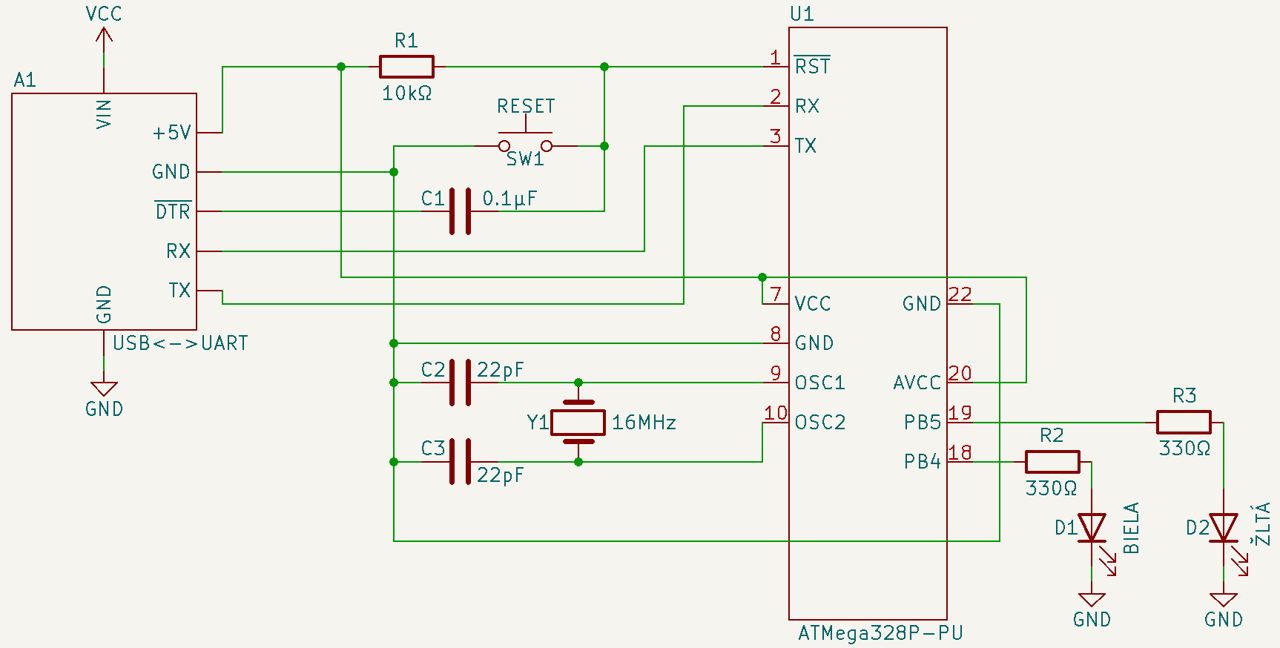
\includegraphics[width=1\textwidth]{images/schemeATMega.png}}
    \caption[Schéma zapojenia mikrokontroléra ATMega328P.]{Schéma zapojenia mikrokontroléra ATMega328P.}
    \label{obr:schemeATMega}
\end{figure}